\documentclass[aspectratio=169]{beamer}
\usetheme{UniBern}
\title{Tomographic imaging of fish}
\subtitle{Or how to image much, \emph{much} more teeth}
\author{David Haberthür}
\institute{Institute of Anatomy\\Universität Bern}
\date{January 18, 2024 | Seminar@Institute of Anatomy}

% Some often used abbreviations/commands
\newcommand{\everyframe}{1}% use only every nth frame for the animations
\newcommand{\imagewidth}{\columnwidth}% set global image width
\newcommand{\imageheight}{0.618\paperheight}% set global image heidht
\newlength\imagescale% needed for scalebars
\newcommand{\uct}{{\textmu}CT\xspace}% make our life easier
\newcommand{\eg}{e.\,g.\xspace}%
\newcommand{\ie}{i.\,e.\xspace}%

\usepackage[backend=biber,
	style=numeric,
	url=false,
	isbn=true,
	maxnames=1,
	sorting=none]{biblatex}
\addbibresource{../../Documents/library.bib} % FastSSD, Windows or Mac works (on Linux/FastSSD we generated a 'Document' folder at the correct level and `ln -s ~/P/Documents/library.bib .` to it)
\usepackage{tikz}
	\usetikzlibrary{shadows,spy}
	\tikzset{shadowed/.style={preaction={transform canvas={shift={(1pt,-1pt)}},draw=ubRed}}}
\usepackage{shadowtext}
	\shadowoffset{1pt}
	\shadowcolor{ubRed}
\usepackage{pgfplots}
	\pgfplotsset{compat=newest}
\usepackage{microtype}
\usepackage[detect-all=true,
	range-phrase=--,
	range-units=single,
	per-mode=symbol,
	per-symbol=/]{siunitx}
\usepackage[absolute,overlay]{textpos}
\usepackage[showseconds=false,showzone=false]{datetime2}
\usepackage{gitinfo2}
\usepackage{xspace}
\usepackage{ccicons}
\usepackage[version=4]{mhchem}
\usepackage{animate}
\usepackage{listings}
	\lstset{basicstyle=\scriptsize\ttfamily}
	% highlight a line in listings: https://tex.stackexchange.com/a/58543/828
	% Including a crude workaround for recent versions of `listings`: https://tex.stackexchange.com/a/451538/828
	\makeatletter%
	\let\old@lstKV@SwitchCases\lstKV@SwitchCases%
	\def\lstKV@SwitchCases#1#2#3{}%
	\makeatother%
	\usepackage{lstlinebgrd}%
	\makeatletter%
	\let\lstKV@SwitchCases\old@lstKV@SwitchCases%
	\lst@Key{numbers}{none}{%
		\def\lst@PlaceNumber{\lst@linebgrd}%
		\lstKV@SwitchCases{#1}%
		{none:\\%
		left:\def\lst@PlaceNumber{\llap{\normalfont%
		\lst@numberstyle{\thelstnumber}\kern\lst@numbersep}\lst@linebgrd}\\%
		right:\def\lst@PlaceNumber{\rlap{\normalfont%
			\kern\linewidth{}\kern\lst@numbersep%
			\lst@numberstyle{\thelstnumber}}\lst@linebgrd}%
		}{\PackageError{Listings}{Numbers #1 unknown}\@ehc}}%
	\makeatother%
	% highlight a line in listings: https://tex.stackexchange.com/a/58543/828
\usepackage{pgfplotstable}
\usepackage{booktabs}
\usepackage{colortbl}
\usepackage{mathastext}
\usepackage{lipsum}

% change tikz font to slide font
% https://tex.stackexchange.com/a/33329/828
\usepackage[eulergreek]{sansmath}
\pgfplotsset{tick label style = {font=\sansmath\sffamily},
	every axis label = {font=\sansmath\sffamily},
	legend style = {font=\sansmath\sffamily},
	label style = {font=\sansmath\sffamily}
}

% Globally thicker lines in with tikz
% https://tex.stackexchange.com/a/206769/828
\tikzset{every picture/.style={thick}}

% Define a custom footer *with* progress bar, based on https://tex.stackexchange.com/a/59749/828
\makeatletter%
\def\progressbar@progressbar{}% the progress bar
\newcount\progressbar@tmpcounta% auxiliary counter
\newcount\progressbar@tmpcountb% auxiliary counter
\newdimen\progressbar@pbht%progressbar height
\newdimen\progressbar@pbwd%progressbar width
\newdimen\progressbar@rcircle% radius for the circle
\newdimen\progressbar@tmpdim% auxiliary dimension
\progressbar@pbwd=0.75\paperwidth%
\progressbar@rcircle=1.5pt%
\def\progressbar@progressbar{%
	\progressbar@tmpcounta=\insertframenumber%
	\progressbar@tmpcountb=\inserttotalframenumber%
	\progressbar@tmpdim=\progressbar@pbwd%
	\multiply\progressbar@tmpdim by \progressbar@tmpcounta%
	\divide\progressbar@tmpdim by \progressbar@tmpcountb%
		\hfill%
		\begin{tikzpicture}%
			\draw[ubGrey] (0,0) -- ++ (\progressbar@pbwd,0);%
			\draw[draw=ubRed,fill=ubGrey] (\the\dimexpr\progressbar@tmpdim-\progressbar@rcircle\relax,.5\progressbar@pbht) circle (\progressbar@rcircle);%
		\end{tikzpicture}%
		\hfill%
		bit.ly/ana-smnr-24\xspace|%
		\xspace v.~\href{https://github.com/habi/Talk.2024.AnatomyInternalSeminar/commit/\gitHash}{\gitAbbrevHash}\xspace|%
		\xspace p.~\insertframenumber/\inserttotalframenumber%
\vspace{0.5ex}%
}%
\addtobeamertemplate{footline}{}%
{%
	\begin{beamercolorbox}[wd=\paperwidth,center]{white}%
		\progressbar@progressbar%
	\end{beamercolorbox}%
}%
\makeatother%

% Format bibliography for beamer
% http://tex.stackexchange.com/a/10686/828
\renewbibmacro{in:}{}
% http://tex.stackexchange.com/a/13076/828
\AtEveryBibitem{%
	\clearfield{journaltitle}
	\clearfield{pages}
	\clearfield{volume}
	\clearfield{number}
	\clearname{editor}
	\clearfield{issn}
	\clearfield{year}
}%
% No parentheses around the (now empty) year: https://tex.stackexchange.com/a/147537/828
\renewcommand{\bibopenparen}{\addcomma\addspace}
\renewcommand{\bibcloseparen}{\addcomma\addspace}

% Acknowledge images just below them
% Based on https://tex.stackexchange.com/a/282637/828
\newcommand{\source}[2]{%
	% Print out (short) link under image, with small text
	\raisebox{-1.618ex}{%
		\makebox[0pt][r]{%
			\tiny\href{http://#1}{#1} #2%
			}%
		}%
	}%
\newcommand{\sourcecite}[2]{%
	% Cite (an image from) a reference
	\raisebox{-1.618ex}{%
		\makebox[0pt][r]{%
			\tiny From~\cite{#1}, #2%
			}%
		}%
	}%
\newcommand{\sourcelink}[3]{%
	% Make the source command an \href{link}{text}
	\raisebox{-1.618ex}{%
		\makebox[0pt][r]{%
			\tiny\href{http://#1}{#2}, #3%
			}%
		}%
	}%

% References as footnotes at the bottom of the slides
% https://tex.stackexchange.com/a/368760/828
\makeatletter
\renewcommand\@makefnmark{\xspace\hbox{\usebeamercolor[fg]{footnote mark}\usebeamerfont*{footnote mark}[\@thefnmark]}}
\renewcommand\@makefntext[1]{\usebeamercolor[fg]{footnote mark}\usebeamerfont*{footnote mark}[\@thefnmark]\enspace\usebeamerfont*{footnote} #1}
\makeatother

\begin{document}
% No footline on the title page
% http://tex.stackexchange.com/a/18829/828 helps us to achieve that
{%
	\setbeamertemplate{footline}{}%
	\begin{frame}[noframenumbering]
		\maketitle
	\end{frame}%
}

% % Alignment frames to test the text-block alignment
% % Mostly here for historic reasons :)
% \begin{frame}{Alignment frame}
% 	\begin{tikzpicture}%
% 		\def\cut{1.75}%
% 		\draw [->] (0,\cut) -- (0.0,\textheight-\cut);%
% 		\draw [<->] (0.5\textwidth,\cut) -- (0.5\textwidth,\textheight-\cut);%
% 		\draw [|-|] (\textwidth,\cut) -- (\textwidth,\textheight-\cut);%
% 		\draw [<->] (0,\cut) -- node [midway, above] {(c, cut) -- (textwidth-cut,textheight-cut))} (\textwidth-\cut,\textheight-\cut) ;%
% 	\end{tikzpicture}%
% \end{frame}
%
% \begin{frame}{Alignment frame II}
% \centering%
% \color{red}\rule{0.618\paperwidth}{\paperheight-0.125\paperheight-0.032\paperheight-6ex}%
% \end{frame}
%
% \begin{frame}[allowframebreaks]{Alignment frame III}
% 	\lipsum[1-3]
% \end{frame}

\begin{frame}
	\frametitle{Grüessech mitenang!}
	\begin{itemize}
		\item David Haberthür
		\begin{itemize}
			\item Physicist by trade
			\item \href{https://boris.unibe.ch/2619/}{PhD in high resolution imaging of the lung}, Institute of Anatomy, University of Bern, Switzerland
			\item Post-Doc I: \href{https://www.psi.ch/sls/tomcat/}{TOMCAT}, \href{https://www.psi.ch/sls/}{Swiss Light Source}, \href{https://www.psi.ch/}{Paul Scherrer Institute}, Switzerland
			\item Post-Doc II: \uct{} group, Institute of Anatomy, University of Bern, Switzerland.
		\end{itemize}
	\end{itemize}
\end{frame}

\begin{frame}
\frametitle{plot}
% Adding plots with TikZ is possible with matplotlib<=3.7 and https://github.com/nschloe/tikzplotlib
% This file was created with tikzplotlib v0.10.1.
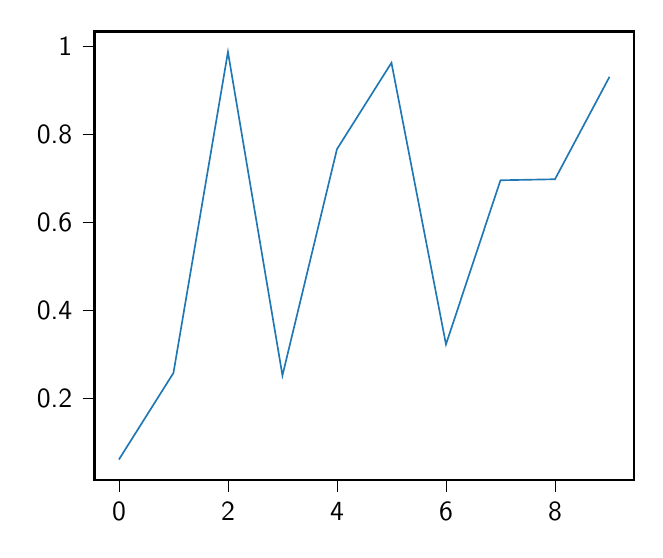
\begin{tikzpicture}

\definecolor{darkgray176}{RGB}{176,176,176}
\definecolor{steelblue31119180}{RGB}{31,119,180}

\begin{axis}[
tick align=outside,
tick pos=left,
x grid style={darkgray176},
xmin=-0.45, xmax=9.45,
xtick style={color=black},
y grid style={darkgray176},
ymin=0.013833521201745, ymax=1.03270328737825,
ytick style={color=black}
]
\addplot [semithick, steelblue31119180]
table {%
0 0.060145783300677
1 0.256795437174552
2 0.986391025279316
3 0.25118122321444
4 0.765474296606782
5 0.961804418862131
6 0.32185355704589
7 0.69478314930869
8 0.697109845085167
9 0.929885276873134
};
\end{axis}

\end{tikzpicture}

\end{frame}

\begin{frame}
\frametitle{plot}
Some text\footnote{doi:10/gsst8t}\\
Some text\footcite{Haberthuer2023}
\end{frame}

\end{document}

\begin{frame}
	\frametitle{Grüessech from the \uct-group}
	\centering
	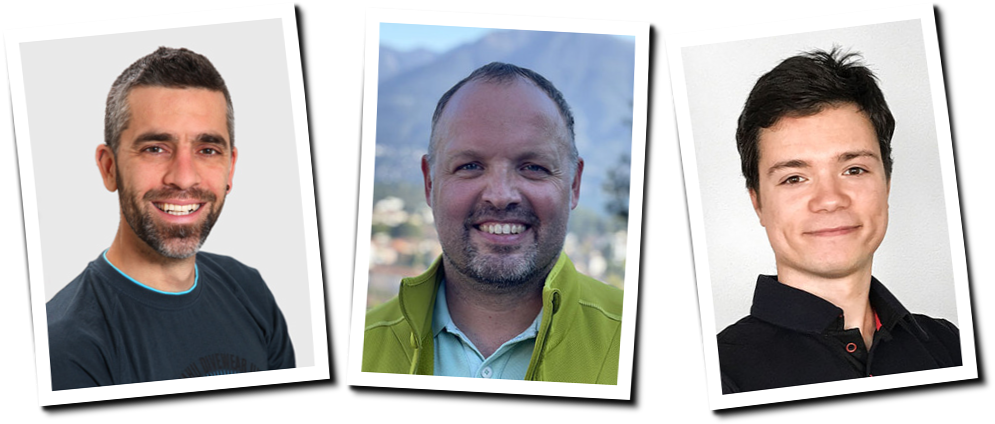
\includegraphics[height=\imageheight]{./images/team}
		\begin{columns}
		\hfill\begin{column}{0.33\textwidth}
			\centering%
			David{\color{ubRed!61.8}.}Haberthuer{\color{ubRed!61.8}@unibe.ch}%
		\end{column}
		\begin{column}{0.33\textwidth}
			\centering%
			Ruslan{\color{ubRed!61.8}.}Hlushchuk{\color{ubRed!61.8}@unibe.ch}%
		\end{column}
		\begin{column}{0.33\textwidth}
			\centering%
			Oleksiy{\color{ubRed!61.8}.}Khoma{\color{ubRed!61.8}@unibe.ch}%
		\end{column}\hfill%
	\end{columns}
\end{frame}

\renewcommand{\imagewidth}{\columnwidth}
\begin{frame}
	\frametitle{\uct-group}
	\begin{columns}
		\begin{column}{0.62\textwidth}
			\begin{itemize}
				\item microangioCT~\cite{Hlushchuk2018}
				\begin{itemize}
					\item Angiogenesis: heart, musculature~\cite{Nording2021} and bones
					\item Vasculature: (mouse) brain~\cite{Hlushchuk2020}, (human) nerve scaffolds~\cite{Wuthrich2020}, (human) skin flaps~\cite{Zubler2021} and tumors
				\end{itemize}
				\item Zebrafish musculature and gills~\cite{MesserliAaldijk2020}
				\item (Lung) tumor detection and metastasis classification~\cite{Trappetti2021}
				\item Collaborations with museums~\cite{Bochud2021} and scientist at UniBe~\cite{Halm2021,Kadlag2023} to scan a wide range of specimens, from human hearing bones to meteorites
				\item Automate \emph{all} the things!~\cite{Haberthuer2021,Haberthuer2023}
			\end{itemize}
		\end{column}%
		\begin{column}{0.38\textwidth}%
			\centering%
			\includegraphics<1|handout:0>[width=\imagewidth]{./images/1172}%
			\only<1|handout:0>{\source{brukersupport.com}{}}%
			\includegraphics<2|handout:1>[width=\imagewidth]{./images/1272}%
			\only<2|handout:1>{\source{bruker.com/skyscan1272}{}}%
			\includegraphics<3|handout:0>[width=\imagewidth]{./images/2214}%
			\only<3|handout:0>{\source{bruker.com/skyscan2214}{}}%
		\end{column}%
	\end{columns}%
\end{frame}

\begin{frame}[allowframebreaks]
	\frametitle{References}
	\renewcommand*{\bibfont}{\scriptsize}
	\setbeamertemplate{bibliography item}{\insertbiblabel}
	\printbibliography{}
\end{frame}

\end{document}
